
%(BEGIN_QUESTION)
% Copyright 2006, Tony R. Kuphaldt, released under the Creative Commons Attribution License (v 1.0)
% This means you may do almost anything with this work of mine, so long as you give me proper credit

Suppose two storage tanks of different size both hold gas at the same low pressure (less than 1 PSI), with no liquid at all:

$$\includegraphics[width=15.5cm]{i00029x01.eps}$$

Use the Ideal Gas Law ($PV = nRT$) to determine what will happen to these two tanks' gas pressures as both tanks become heated by sunlight later in the day.  Assume their gas pressures were equal when both tanks were cold (ambient temperature in the early morning), and that both tanks are perfectly sealed (no gas entering or exiting as the tanks warm).  Choose the best answer matching your prediction:

\vskip 10pt

\begin{itemize}
\item{} Both tanks' pressures will increase, tank A's pressure increasing more than tank B's
\vskip 5pt
\item{} Both tanks' pressures will increase, tank B's pressure increasing more than tank A's 
\vskip 5pt
\item{} Both tanks' pressures will increase by the same amount 
\vskip 5pt
\item{} Tank A's pressure will increase while tank B's pressure will decrease
\vskip 5pt
\item{} Tank B's pressure will increase while tank A's pressure will decrease
\vskip 5pt
\item{} Both tanks' pressures will decrease by the same amount 
\vskip 5pt
\item{} Both tanks' pressures will decrease, tank A's pressure decreasing more than tank B's
\vskip 5pt
\item{} Both tanks' pressures will decrease, tank B's pressure decreasing more than tank A's 
\end{itemize}

\vfil

\underbar{file i00029}
\eject
%(END_QUESTION)





%(BEGIN_ANSWER)

This is a graded question -- no answers or hints given!

%(END_ANSWER)





%(BEGIN_NOTES)

If both tanks begin at the same temperature and the same pressure, we must conclude that the molecular quantity of gas inside each tank is proportional to its interior volume.  For the sake of simple illustration, we could say that tank B has three times as much volume as tank A, and that tank B correspondingly stores three times as many gas molecules as tank A.  That being the case, increasing the temperature of both tanks equally will mean their pressures will rise equally.  Therefore, the best answer assuming an equal rise in temperature for both tanks is: {\bf Both tanks' pressures will increase by the same amount}

\vskip 10pt

However . . . if we assume these tanks are heated by sunlight over a limited period of time, it is possible to conclude that tank A will warm to a higher temperature than tank B because its volume (mass) to surface area ratio is less.  As the linear dimensions of a tank grow, its surface area grows proportionally with the square of those dimensions while the interior volume grows proportionally with the cube of those dimensions.  This means the smaller of the two tanks (A) will have more sunlight-collecting surface area to gather heat per unit of stored mass, and therefore will heat up faster than the large tank.  If the sun sets before the larger tank has reached the temperature of the smaller tank, then the better answer is: {\bf Both tanks' pressures will increase, tank A's pressure increasing more than tank B's}

%INDEX% Physics, static fluids: ideal gas law

%(END_NOTES)


